\documentclass{llncs}
\usepackage{llncsdoc}
\usepackage[english]{babel}
\usepackage[utf8x]{inputenc}
\usepackage{graphicx}
\usepackage{caption}
\usepackage{pmboxdraw}
\usepackage{color}
\definecolor{darkgray}{rgb}{0.41, 0.41, 0.41}
\definecolor{green}{rgb}{0.0, 0.5, 0.0}
\usepackage{listingsutf8}
\lstset{language=Prolog, 
	numbers=left,
	stepnumber=5,
	firstnumber=1,
	numberfirstline=true,
    basicstyle=\linespread{0.8}\ttfamily,
    keywordstyle=\color{blue}\ttfamily,
	showstringspaces=false,
    stringstyle=\color{red}\ttfamily,
    commentstyle=\color{green}\ttfamily,
	identifierstyle=\color{darkgray}\ttfamily,
	tabsize=1,
    breaklines=true,
    extendedchars=true,
	inputencoding=utf8x,
    escapeinside={\%*}{*)},
}
\lstset{literate=%
{↑}{{$\uparrow}$}1
{→}{{$\rightarrow}$}1
{↓}{{$\downarrow}$}1
{←}{{$\rightarrow}$}1
{│}{{$\textSFxi$}}1
{─}{{$\textSFx}$}1
{┌}{{$\textSFi}$}1
{┬}{{$\textSFvi}$}1
{┐}{{$\textSFiii}$}1
{├}{{$\textSFviii}$}1
{┼}{{$\textSFv}$}1
{┤}{{$\textSFix}$}1
{└}{{$\textSFii}$}1
{┴}{{$\textSFvii}$}1
{┘}{{$\textSFiv}$}1
}

\setlength{\tabcolsep}{6pt}

\begin{document}

\title{Solving the Puzzle Magnets with Constraint Logic Programming}
\author{\^Angela Cardoso \and Nuno Valente}
\institute{FEUP-PLOG, Turma 3MIEIC02, Grupo Magnets\_2.}
\maketitle


\begin{abstract}
	
	This project was developed as part of the coursework for the subject of Logic Programming at the Faculty of Engineering of the University of Porto. In order to learn logic programming with constraints, we chose the puzzle Magnets to implement in SICStus Prolog. The application obtained is capable of solving a given Magnets puzzle, as long as it is supplied in a specific format, generating random puzzles of the required size and displaying both the puzzle and the solution in a user friendly text format. The efficiency of the solution we obtained depends, of course, on the size of the puzzle, but more so on its degree of difficulty. One can easily obtain puzzles where the constraints do not allow for immediate variable reduction, which leads to frequent backtracking and thus long execution times. There is also a lot of symmetry in theses puzzles, which in a straightforward implementation often increments the difficulty of reaching a solution. 
	
\end{abstract}


\section{Introduction}

Constraint logic programming is very useful to solve problems in which one wants to determine a set of variables that must satisfy certain rules. In addition to the the logic programming literals, these programs contain constraints such as~$X \neq Y$. The goal of the program is to determine values for all the variables such that all the clauses and constraints are satisfied. Typically, this kind of programming is used to solve search problems, such as paper-and-pencil puzzles or chess puzzles, and optimization problems, such as scheduling, timetabling, resource allocation, planning, production management or circuit check. By using constraint logic programming one can reduce the development time, as well as obtain efficient, simple and easy to maintain solutions.

To solidify our knowledge of constraint logic programming, we chose to implement the paper-and-pencil puzzle Magnets. In this puzzle, one is given a square grid of dominoes, as well as the number of positive and negative poles for each row and column. Some dominoes are magnetized, having a positive pole and a negative pole, while others are neutral. Also, poles with the same charge repel and are not allowed to touch vertically or horizontally. The objective is identify the positive poles with a $+$ sign, the negative poles with a~$-$ sign and the neutral ones with an~$x$.

The following sections describe the progress of our work on this subject, with details of our implementation and of the results we obtained, including statistics that give some insight to the quality of our solution.

%Descricao dos objetivos e motivacao do trabalho, referencia sucinta ao problema em analise (idealmente, referencia a outros trabalhos sobre o mesmo problema e sua abordagem), e descricao sucinta da estrutura do resto do artigo.


\section{Problem Description} 

Although we managed to find several online implementations or descriptions of the Magnets puzzle, we could not determine its origins. In any case, the rules are quite clear:
\begin{itemize}
	\item for each row and each column the number of positive and negative poles must be as specified;
	\item each charged domino must have a positive and a negative pole;
	\item two positive, or two negative, charged poles must not be vertically or horizontally adjacent.
\end{itemize}
Figure~\ref{example} illustrates these rules, showing a solved Magnets puzzle.

\begin{figure}[htbp]
\begin{center}
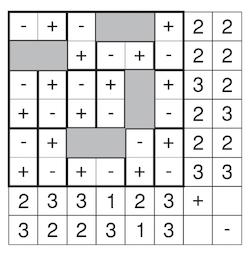
\includegraphics[scale=0.6]{magnets.jpg}
\caption{Example of a Magnets puzzle}
\label{example}
\end{center}
\end{figure}

Our objective is to use constraint logic programming to implement a Magnets puzzle solver. Theoretically, our implementation should be able to handle any such puzzle. However, the exponential nature of such puzzles will certainly impose limitations on any devised implementation. Hence, it is also our intent to obtain an efficient method to solve these puzzles.


\section{Approach}

Even a casual observation of the rules of Magnets gives some clue that this puzzle is suited for constraint logic programming. We shall make this clear in the following sections, where we present a formal description of Magnets as a constraint satisfaction problem (CSP).

\subsection{Decision Variables} 

In any CSP there are variables whose value we aim to determine. For Magnets, the decision variables are the half dominoes or poles, that is, each small square in the grid is a decision variable. In order to solve the puzzle, we must obtain the value (positive, negative or neutral) of each of these poles. To better represent these values, and in order to allow for constraint resolution in SICStus Prolog, we used the following conversions:
\begin{itemize}
	\item 1 represents positive poles;
	\item -1 represents negative poles;
	\item 0 represents neutral poles. 
\end{itemize}

Since Magnets puzzles are square grids of a given size~$N$, the number of decision variables is~$N^2$. Each of these variables has 3 possible values, therefore there is a total of $3^{N^2}$ possible solutions to be tested. These variables are organized sequentially in a list from top of the grid to bottom and from left to right.

\subsection{Constraints} 

For each Magnets rule, there is a rigid constraint in our Magnets CSP. The first restriction is on the number of positive and negative poles for each row and column. In order to implement this in SICStus Prolog, we used the combinatorial constraint \verb|global_cardinality|. First we organize our puzzle as a list of rows, then we use \verb|global_cardinality| to force each row to have a specific number of~$1s$,~$0s$ and~$-1s$. Afterwards, the same thing is done for the columns.

The second rule forces each charged domino or magnet to have a positive and a negative pole. This is done with a simple arithmetic constraint. Given our codification of positive, negative and neutral, the sum of both poles of a magnet must be zero. Hence, we use the constraint \verb|#=| to enforce this equality.

Finally, there is a rule on the proximity of same charge poles. Two positive (respectively, negative) poles repel each other, therefore, they cannot be vertically or horizontally adjacent. Again, we check this with an arithmetic constraint. Given two neighbor (vertically or horizontally adjacent) poles, the sum of their cannot be bellow~$-1$ or above~$1$. Indeed, we can only obtain~$2$ if there are two positive adjacent poles, and the same thing for~$-2$ and negative poles. Hence, we use the constraints \verb|#>| and \verb|#<| to verify this last rule.

\subsection{Search Strategy} 

In order to attribute values to the variables, SICStus uses the predicate labeling, for which one may provide some options that, depending on the problem at hand, may increase the efficiency of the search for a solution. In our implementation of Magnets, these options where mainly chosen through trial and error. In fact, we started by using no options at all (which is the same as using the default options) and then, with a collection of somewhat difficult puzzles, we determined the options with better time performance. 

The first option to consider is variable ordering. That is, which variable should be first consider when Prolog tries to find a possible solution. The default option starts with the leftmost variable, in our case, the first square of the grid. There are several other options that we will not exhaustively mention, because we quickly concluded that they are not suitable for our problem. Besides \verb|leftmost| the ones we tested where:
\begin{itemize}
	\item \verb|first_fail|, which chooses the leftmost variable with the smallest domain;
	\item \verb|occurrence|, which chooses the leftmost variable with the largest number of constraints;
	\item \verb|ffc|, which combines first \verb|first_fail| and \verb|occurrence|.
\end{itemize}
The performance of these options is not always consistent, that is, the better option depends on the specific example. However, in our limited experiments, there seems to be an advantage for \verb|leftmost|, even though sometimes \verb|first_fail| is better. Ordering options including \verb|occurrence| did not perform well in our examples. This is probably due to the fact that the number of restrictions on each variable is more or less the same, with the exception being the extremes of the puzzle, since they have less neighbors. In the end, we opted to use the default \verb|leftmost|, because there is some limited evidence of its superiority.

The next option is about value selection. Given a variable and a set of possible values for that variable, how should Prolog decide which one to try first. We also made some experiments with these options, but we quickly decided on the best one. Indeed, there are at most three possible values for a Magnets variable:~$-1$,~$0$ and~$1$. For every~$-1$ there is a~$1$, because of the second rule, that is, the total number of~$-1s$ is the same as the total number of~$1s$. On the other hand,~$0s$ come in pairs, since every neutral domino must have two of them. This means that in a puzzle where there is some equilibrium between the number of neutral and charged dominoes, there will be approximately twice as much~$0s$ as~$-1s$ or~$1s$. This means that the average randomly generated puzzle has more~$0s$ and thus, we are more likely to succeed if we try~$0$ first. With this reasoning in mind we chose the option \verb|median| for value selection, since for every variable with domain~$\{-1, 0, 1\}$ this will lead to~$0$ being chosen first.

Once~$0$ has been tested, given the puzzle symmetry, there is no advantage in trying~$-1$ or~$1$ first, therefor we chose no option for value ordering, which means that the default \verb|up| is used.

To test these options we ran the same 1000 random puzzles of size 10, with different sets of options. The average time using the default options was 25 seconds, with \verb|first_fail| the time was 28 seconds, with \verb|median| 23 seconds, and with both \verb|first_fail| and \verb|median| 36 seconds. Although these results have very slight variations, the maximum time is quite more telling, with 1410 seconds for the defaults, 3360 seconds for \verb|first_fail|, 870 seconds for \verb|median| and 5360 seconds for both \verb|first_fail| and \verb|median|. These were the results that influenced our decision in the final application.


\section{Puzzle Generation}

In order to test our Magnets solver, we decided to implement a random Magnets puzzle generator. Given a positive even integer, this generator creates a random Magnets puzzle of that size, for which there is at least one solution. As it turns out, this is also an adequate problem to solve with constraint logic programming. Indeed, to have a valid Magnets puzzle, we need a square grid of dominoes, as well as the number of negative and positive poles in each row and each column. As in the previous section we will now formalize the description of Magnets puzzle generation as a CSP, but we will do so in a more succinct manner. In particular, we used no labeling options other than the default, so there is no subsection about that.

\subsection{Decision Variables} 

In order to obtain a Magnets puzzle, first we need the square grid of dominoes. In our implementation we represent each cell of the grid with a cardinal point (\verb|n|, \verb|s|, \verb|e| or \verb|w|), that points to the other half of its domino. Thus, the list of half dominoes forms our first set of variables. Since SICStus Prolog demands small integer domains constraint resolution, our program actually uses integers from~$1$ to~$4$ to represent the cardinal points, but after these variables are assigned they are translated to the letters above.

Besides the grid of dominoes, Magnets also has lists with the numbers of positive and negative poles for each row and column. These lists form the rest of our decision variables. If the puzzle has size~$N$, then we have four lists, each with~$N$ integers whose domain is~$\left[0, N\right]$. Thus, in total we have~$N^2 + 4N$ variables to generate a Magnets puzzle of size~$N$.

\subsection{Constraints} 

The first constraints we need to consider are those that allow us to obtain a suitable set of dominoes. These dominoes cannot overlap and they must fill the entire square. If we starting from the top left corner, going to the right and then to the bottom, it is not hard to guarantee the no overlap rule. All we have to do is, for each new domino, chose either the east or the south direction. Unless we are at a border, then only one of these is available. 

However, as we get closer to the bottom of the square, we may find ourselves trapping a single cell, which contradicts the rule of filling the whole grid with dominoes. To overcome this, we still let Prolog chose randomly between east and south for new dominoes, but we add a constraint that states that for each half domino has a corresponding half with opposite direction. Since all cells of the grid must have a direction, Prolog then uses backtracking to verify this constraint and obtain a suitable grid. 

The real trick here is to chose the next value randomly, instead of with some prefixed order has is with all labeling options. To obtain this random effect, we added redundant constraints and used random asserts and retracts to establish the order in which the satisfaction of these constraints is attempted.

After obtaining the grid of dominoes, we fill that grid with the values~$-1$,~$0$ and~$1$, applying the same constraints from the puzzle solution, that is, the sum of both poles of a magnet must be zero and the sum of two vertically or horizontally adjacent poles is at least~$-1$ and at most~$1$. Once this is done, we compute the number of negative and positive poles in each row and column by simply counting them.


\section{Solution Presentation} 

In addition to random puzzle generation and puzzle resolution, we also implemented some Prolog predicates that allow us tu visualize the puzzles and the solutions in text mode. In fact, we have a very small application that asks the user for the size of the puzzle, shows a random puzzle of that size and then, when the user choses to, presents the solution. 

\begin{figure}[htbp]
\begin{center}
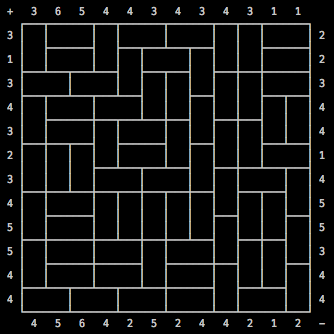
\includegraphics[scale=0.6]{puzzle.png}
\caption{The display of a Magnets puzzle}
\label{puzzle}
\end{center}
\end{figure}

Figure~\ref{puzzle} shows the output of the puzzle display predicate for a size 12 puzzle, while Figure~\ref{result} shows the solution of the same puzzle.
 
\begin{figure}[htbp]
\begin{center}
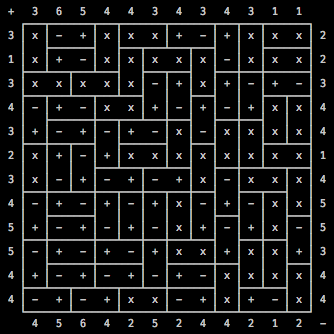
\includegraphics[scale=0.6]{result.png}
\caption{The display of a solved Magnets puzzle}
\label{result}
\end{center}
\end{figure}

The predicates used to obtain these outputs just go through the puzzle and the result, both represented as lists of rows, and draw the grid and its contents. The hardest part is to use the correct box drawing characters depending on the position of each domino.

\section{Results}

We used our random puzzle generator and some of SICStus statistics predicates to test the efficiency of the solver. Since the time varies a lot between different puzzles of the same size, we computed, in addition to the average run time, the minimum and the maximum. We also tracked the average number of backtracks for puzzle solving. The results are presented in Table~\ref{table}, with the time measured in seconds.

\begin{center}
\begin{tabular}{ | l || c | c | c | c | c | c | }
	\hline
	Puzzle Size 	&	2.00	&	4.00	&	6.00	&	8.00	&	10.00	&	12.00	\\\hline
	Minimum Time	&	0.00	&	0.00	&	1.00	&	2.00	&	3.00	&	6.00	\\\hline
	Average Time	&	0.34	&	1.08	&	2.26	&	5.27	&	19.90	&	865.47	\\\hline
	Maximum Time	&	6.00	&	13.00	&	28.00	&	81.00	&	353.00	&	20609.00	\\\hline
	Average Backtracks	&	0.00	&	0.16	&	0.94	&	7.54	&	207.64	&	13998.90	\\\hline
\end{tabular}
\captionof{table}{Magnets solution efficiency}
\label{table}
\end{center}

Using a logarithmic scale of base 3, which is appropriate since everything points to an exponencial time complexity, we obtained from Table~\ref{table} the graph in Figure~\ref{chart}, where the puzzle sizes range from 2 to 12.

\begin{figure}[htbp]
\begin{center}
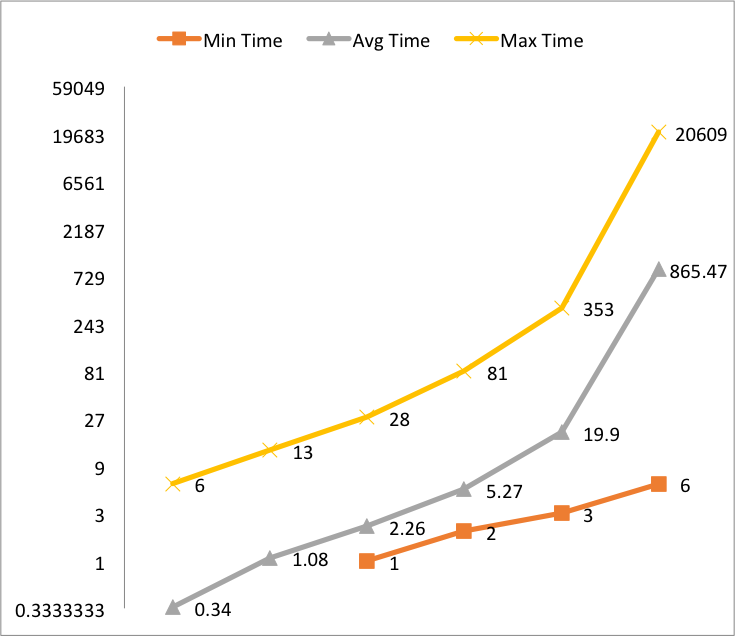
\includegraphics[scale=0.7]{chart.png}
\caption{Time to solve a Magnets puzzle}
\label{chart}
\end{center}
\end{figure}

Due to time constraints, these tests where performed in samples of 100 puzzles and we could not finish the test for 100 puzzles of size 14. But with the time differences observed in same size puzzles, we do not put much trust in these results. More robust tests should be performed in a powerful machine that could be left running the puzzles for a long time. That way, it would be possible to obtain bigger samples and with larger sizes, leading to an experimental conjecture for time complexity of our solver.


\section{Conclusions and Future Work} 

This project allowed us to better understand constraint logic programming and how well suited it is for puzzle solving. In fact, 
the use of Prolog and in particular of constraints made this task much simpler than it would have been with other languages or tools.

In the end our implementation is very close to the rules of the puzzle Magnets, with only some translations and improvements that allow us to avoid symmetry. We did try to think of other redundant constraints that could improve the results. However none of our ideas has materialized. This would be one of the lines for continuing this work, to use a more sophisticated constraint program that can reduce the time to compute a solution.

Even tough our tests where limited, the results seem to point to exponential complexity, in fact the theoretical number~$3^{N^2}$ is in agreement with the run times we obtained experimentally. Of course, further tests should be conducted, with bigger samples and larger puzzles, in order to comprove these initial results.

Depending on the puzzle, our solver can reach a solution quite fast, even for larger puzzles, but the fact that the time varies so much makes it somewhat unreliable. However, for the casual user, with puzzles of size up to 10, the application should have no problem in computing the solution in a reasonable amount of time. At sizes 14 and above its a trial and error procedure, some times quite fast and other times excruciatingly slow.


\appendix
\section{Source Code}

\subsection{File magnets.pl}
\lstinputlisting{../src/magnets.pl}

\subsection{File display.pl}
\lstinputlisting{../src/display.pl}

\subsection{File solver.pl}
\lstinputlisting{../src/solver.pl}

\subsection{File generator.pl}
\lstinputlisting{../src/generator.pl}

\subsection{File stats.pl}
\lstinputlisting{../src/stats.pl}

\subsection{File utils.pl}
\lstinputlisting{../src/utils.pl}


\begin{thebibliography}{}

\bibitem{an:to:ni}
Niederlinski, Antoni:
A gentle guide to constraint logic programming
via ECL$^i$PS
Gliwice 2014

\bibitem{guide}
Notes from theoretical classes

\bibitem{site1}
https://sicstus.sics.se/sicstus/docs/3.7.1/html/sicstus\_33.html

\bibitem{site2}
http://www.janko.at/Raetsel/Magnete/index.htm

\bibitem{site3}
http://www.constraintsolving.com/tutorials/cp\-tutorial

\bibitem{site4}
http://www.swi\-prolog.org/man/clpfd.html

\bibitem{site5}
https://en.wikipedia.org/wiki/Box\-drawing\_character

\end{thebibliography}

\end{document}
